\documentclass[10pt]{beamer}
\usetheme{jambro}
\graphicspath{{./graphics/}}

% Authors/institutes/date/etc
%--------------------------------
\title[]{Way Down in the Hole: Adaptation to Long-Term Water Loss in Rural India}
%\subtitle{American Economic Review}
\author[]{David Blakeslee, Ram Fishman, Veena Srinivasan}
\date{\today}

\begin{document}
%=============================================================

\begin{frame}[plain]
	\titlepage{
		\begin{center}
			\begin{minipage}{0.8\textwidth}
				\centering
				\color{title!80}{\scriptsize Roy Kisluk}
			\end{minipage}
		\end{center}}
\end{frame}

%===========================================================

\section{Introduction}
\begin{frame}
	{Introduction}
	\begin{itemize}
		\item Groundwater depletion in southern India %\(\Rightarrow\) adaptation, labor reallocation, income diversification, effects on children%
		\item Why is it important?
		      \begin{itemize}
			      \item Groundwater depletion is a critical threat to agriculture-dependent livelihoods
			      \item Socioeconomic impacts of environmental degradation
			      \item Inform sustainable development policies
		      \end{itemize}
		\item Quasi-random variation in geological factors causing borewell failure as exogenous shock
		\item Compare HH with functional borewells to HH with failed borewells
		\item How do rural households in India adapt to long-term water loss caused by groundwater depletion?
		\item What role does labor reallocation to non-agricultural sectors play in maintaining household income?
	\end{itemize}
\end{frame}
%=============================================================
\begin{frame}
	{Methodology}
	\begin{itemize}
		\item Hard-rock geology: spatially random subsurface pockets \(\Rightarrow\) quasi-random groundwater access
		\item HHs within the same village
		\item Divide HHs into successful or failed first borewell, to avoid confounding effects of wealthier households
		\item Compare outcomes between HHs with currently active and inactive borewells
		\item Specialized cameras confirm geological differences drive borewell failures, validate exogeneity
		\item Robustness tests show no pre-existing correlation between borewell age, depth, or cost and household socioeconomic conditions
		\item Regress outcomes (e.g., income, labor shifts) on borewell failure, using household controls, fixed effects for village and year of drilling
	\end{itemize}
\end{frame}
%=============================================================
\begin{frame}
	{Data}
	\begin{columns}
		% Left column
		\begin{column}{0.7\textwidth}
			\begin{itemize}
				\item Household survey data: 1,408 households from 102 villages in Karnataka that rely primarily on groundwater for irrigation
				\item Data on every borewell drilled, its functionality status, costs, depths, and drilling year
				\item Household characteristics, including cropping patterns, income sources (farm and off-farm), assets
				\item Supplementary village-level data from the 2013 Economic Census, used to measure the presence of firms and local industry
			\end{itemize}
		\end{column}
		\begin{column}{0.3\textwidth}
			\centering
			\begin{figure}
				\centering
				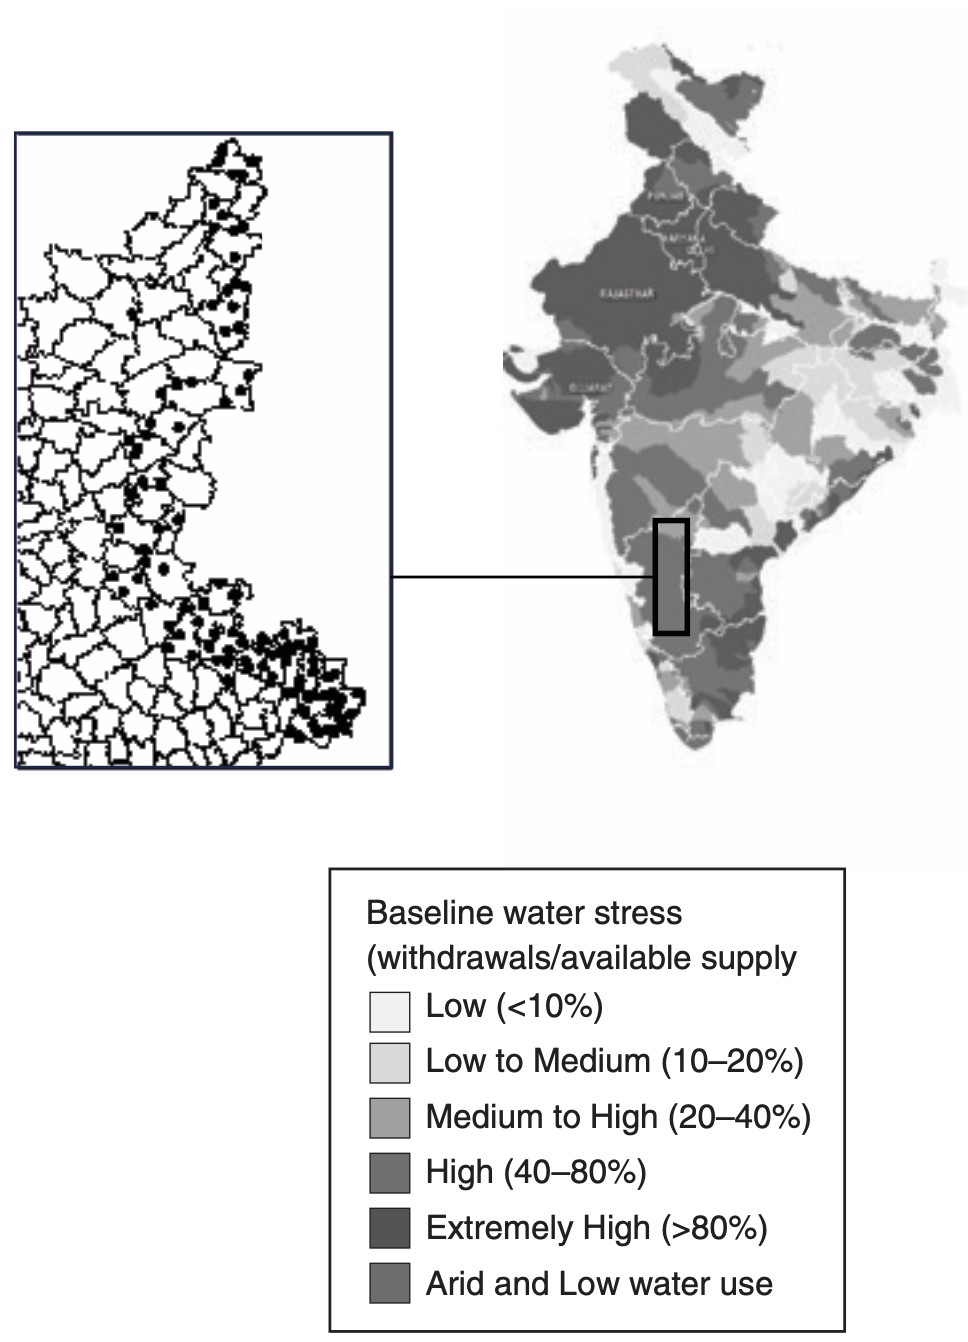
\includegraphics[width=1\textwidth]{figure1_left.png}
				\caption{Baseline water stress (withdrawals/available supply)}
			\end{figure}
		\end{column}
	\end{columns}
\end{frame}

%=============================================================
\begin{frame}
	{Results}
	\begin{itemize}
		\item Significant drop in farm income with no agricultural adaptation
		\item Households shifted labor to off-farm employment to offset income losses, mediated by presence of large firms
		\item Increased debt and asset liquidation
		\item Older children enrollment decreased to supplement income, younger children enrollment increased
	\end{itemize}
\end{frame}

%=============================================================
\begin{frame}
	{Literature Review (in 30 seconds)}
	\begin{itemize}
		\item Detrimental effects of climate change on agricultural livelihoods and social outcomes
		      \begin{itemize}
			      \item Auffhammer et al. 2013
			      \item Dell, Jones, and Olken 2014
			      \item Carleton and Hsiang 2016
		      \end{itemize}
		\item Households' coping strategies in response to transient income shocks, including asset sales, income diversification, and migration
		      \begin{itemize}
			      \item Alderman and Paxson 1994
			      \item Morduch 1995
			      \item Dercon 2002
		      \end{itemize}
		\item Shifts to non-agricultural employment in response to transient weather shocks
		      \begin{itemize}
			      \item Kochar 1999
			      \item Macours, Premand, and Vakis 2012
			      \item Colmer 2016
		      \end{itemize}
		      %\item Conceptual limitations inherent in the use of transient, high-frequency environmental variation for the purpose of studying the impacts of long-term environmental shifts
		      %      \begin{itemize}
		      %	      \item Dell, Jones, and Olken 2014
		      %	      \item Hsiang, 2016
		      %	      \item Carleton and Hsiang 2016
		      %      \end{itemize}
	\end{itemize}
\end{frame}
%=============================================================
\begin{frame}
	{Overview}
	\begin{enumerate}
		\item Background
		\item Data
		\item Empirical Strategy
		\item Results
		\item Conclusion
		\item Thesis
	\end{enumerate}
\end{frame}
%=============================================================
\section{Background}
\begin{frame}
	{Background}
	\begin{columns}
		\begin{column}{0.5\textwidth}
			\begin{itemize}
				\item Groundwater use has grown by 105\% since the 70s, in contrast to 28\% growth in surface water use
				\item Access, use, and depletion is dependent on characteristics of the subsurface hydrogeology
				\item Over-extraction is largely concentrated in two parts of India:
				      \begin{itemize}
					      \item The Northwest, where aquifers are deep and alluvial
					      \item Central-southern India, where aquifers occur within a hard-rock geology
				      \end{itemize}
			\end{itemize}
		\end{column}
		\begin{column}{0.5\textwidth}
			\centering
			\begin{figure}
				\centering
				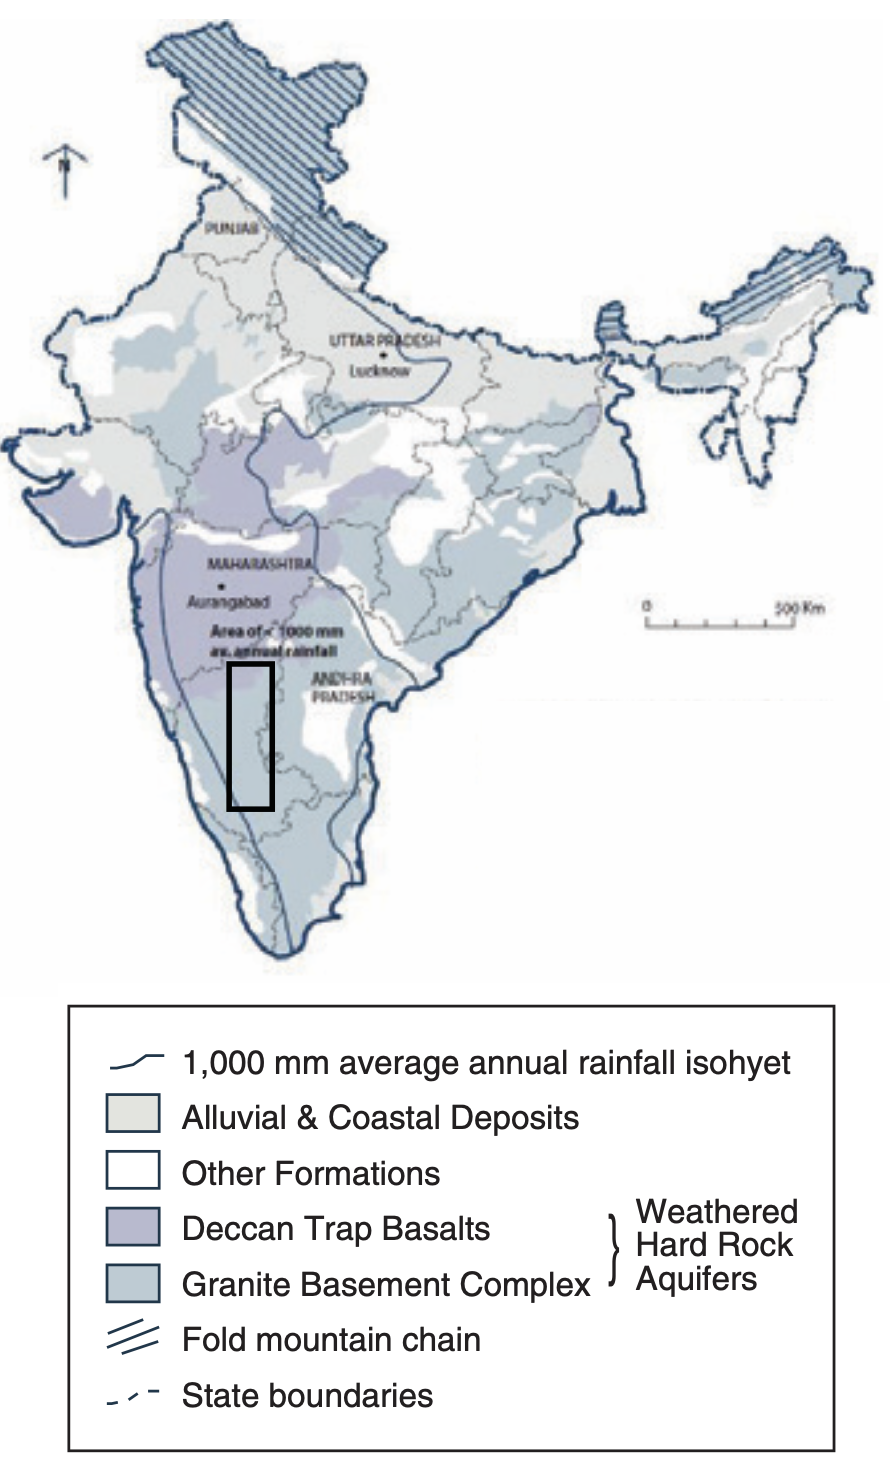
\includegraphics[width=0.5\textwidth]{figure1_right.png}
				\caption{Classification of aquifer systems; light grey shades mark alluvial aquifers, else: hard-rock aquifers}
			\end{figure}
		\end{column}
	\end{columns}
\end{frame}

%=============================================================
\begin{frame}
	{Background}
	\begin{itemize}
		\item Most subsurface consists of impermeable rock with networks of fractures and pockets of permeable material (where groundwater is stored)
		\item Borewells drilled into the hard rock tap into these water-bearing pockets, intersect 0—5 sources; each borewell is just a few decimeters thick
		\item Fractures' exact location and spacing cannot be determined by surface features; their patterns are highly heterogeneous and unpredictable
		\item Until 60s: mostly shallow, dug wells. Late 60s: “down-the-hole” (DTH) drilling enabled access to deeper sources of water at high cost. 90s: rising incomes enabled a proliferation of DTH
	\end{itemize}
	\begin{figure}
		\centering
		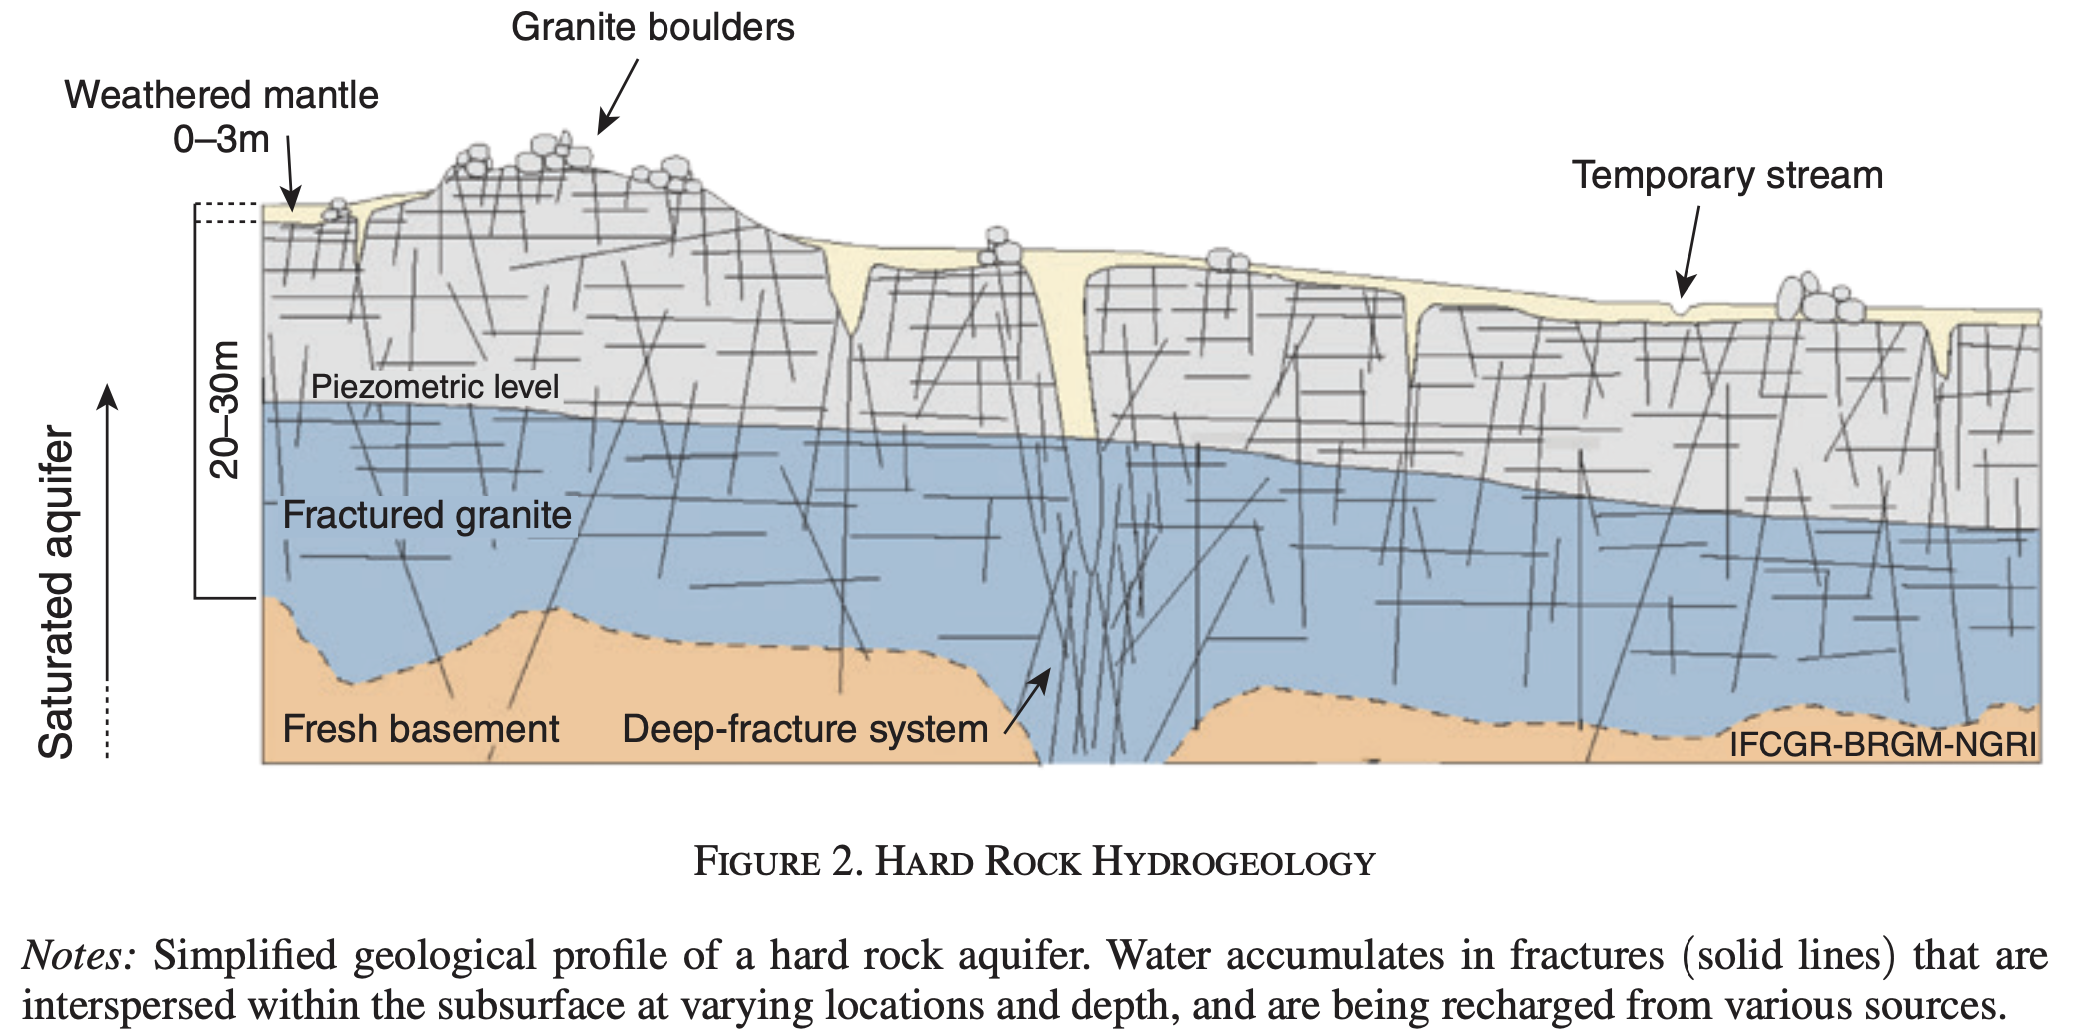
\includegraphics[width=0.5\textwidth]{figure2.png}
	\end{figure}
\end{frame}

%=============================================================
\begin{frame}
	{Background}
	\begin{itemize}
		\item Important to our study:

	\end{itemize}
	\begin{enumerate}
		\item Local aquifers have limited storage, exhaust more rapidly than alluvial aquifers of NW India; water levels dropping since 90s, many dried up
		\item High degree of quasi-random spatial variation, even at small distances, in rate of hitting water and operation time before it dries up
		\item Drilling is costly (more than x2 median household annual income) and a risky investment
	\end{enumerate}
\end{frame}

%=============================================================
\section{Data}
\begin{frame}
	{Data}
	\begin{itemize}
		\item 2016 survey: 1,408 land-owning households from 102 villages randomly selected from 31 districts in Karnataka, not served by surface irrigation
		\item Supplemented with village-level admin data from 2013 Economic Census, which provides information on the number and size of firms within each village and in adjacent area
	\end{itemize}
	\begin{figure}
		\centering
		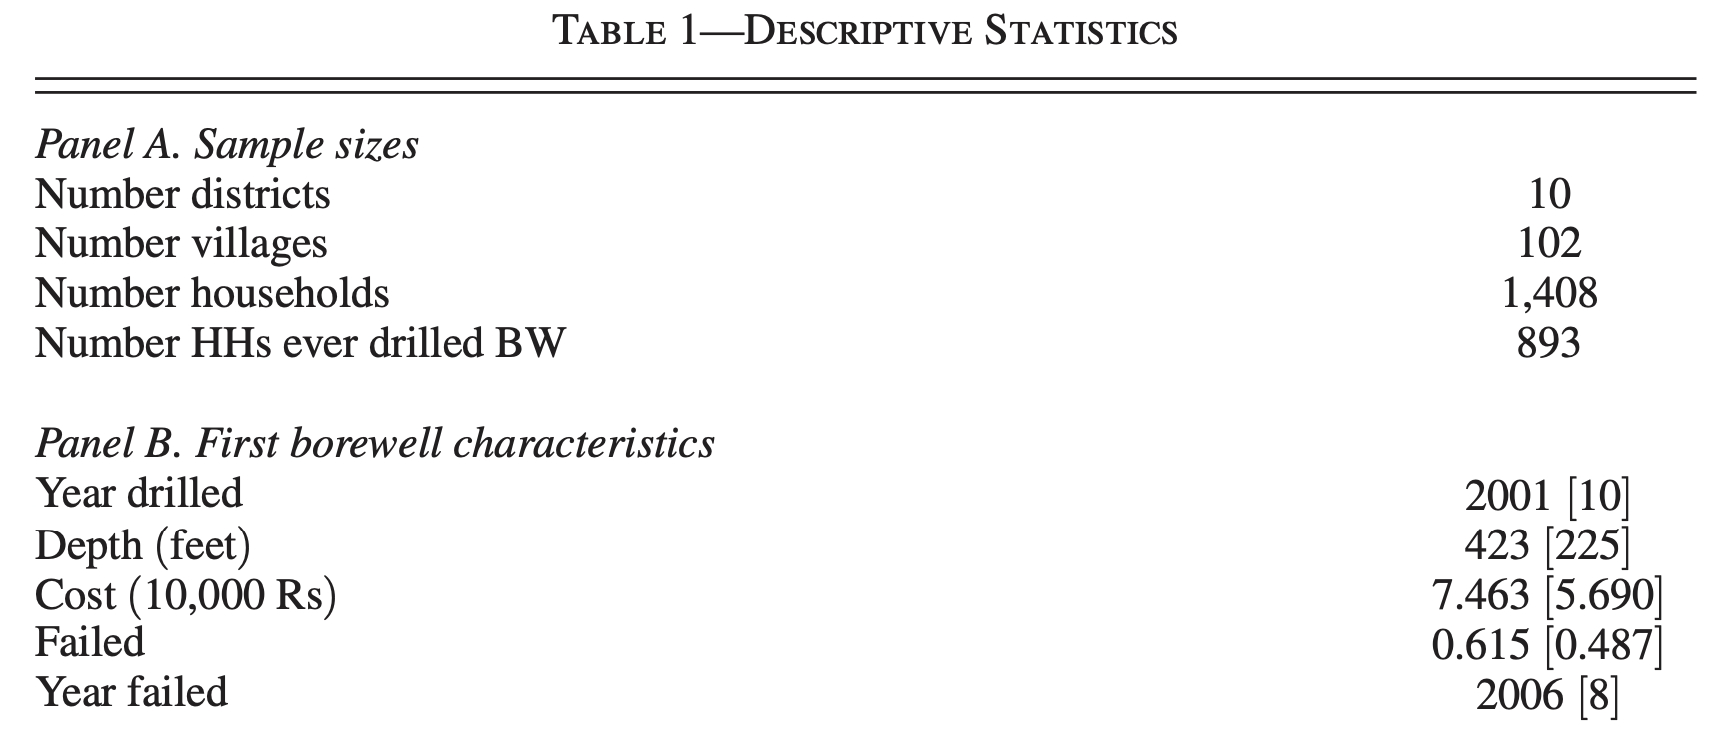
\includegraphics[width=0.8\textwidth]{table1_ab.png}
	\end{figure}
\end{frame}
%=============================================================
\begin{frame}
	{Data}
	\begin{columns}
		\begin{column}{0.4\textwidth}
			\begin{itemize}
				\item Households with functioning borewells have much higher farm and total
				      income, and own more land and other assets
				\item Greater wealth can enable households to retain access to water by drilling more and deeper wells
				\item Therefore, these differences cannot be interpreted as being caused by access to water
			\end{itemize}
		\end{column}
		\begin{column}{0.6\textwidth}
			\begin{figure}
				\centering
				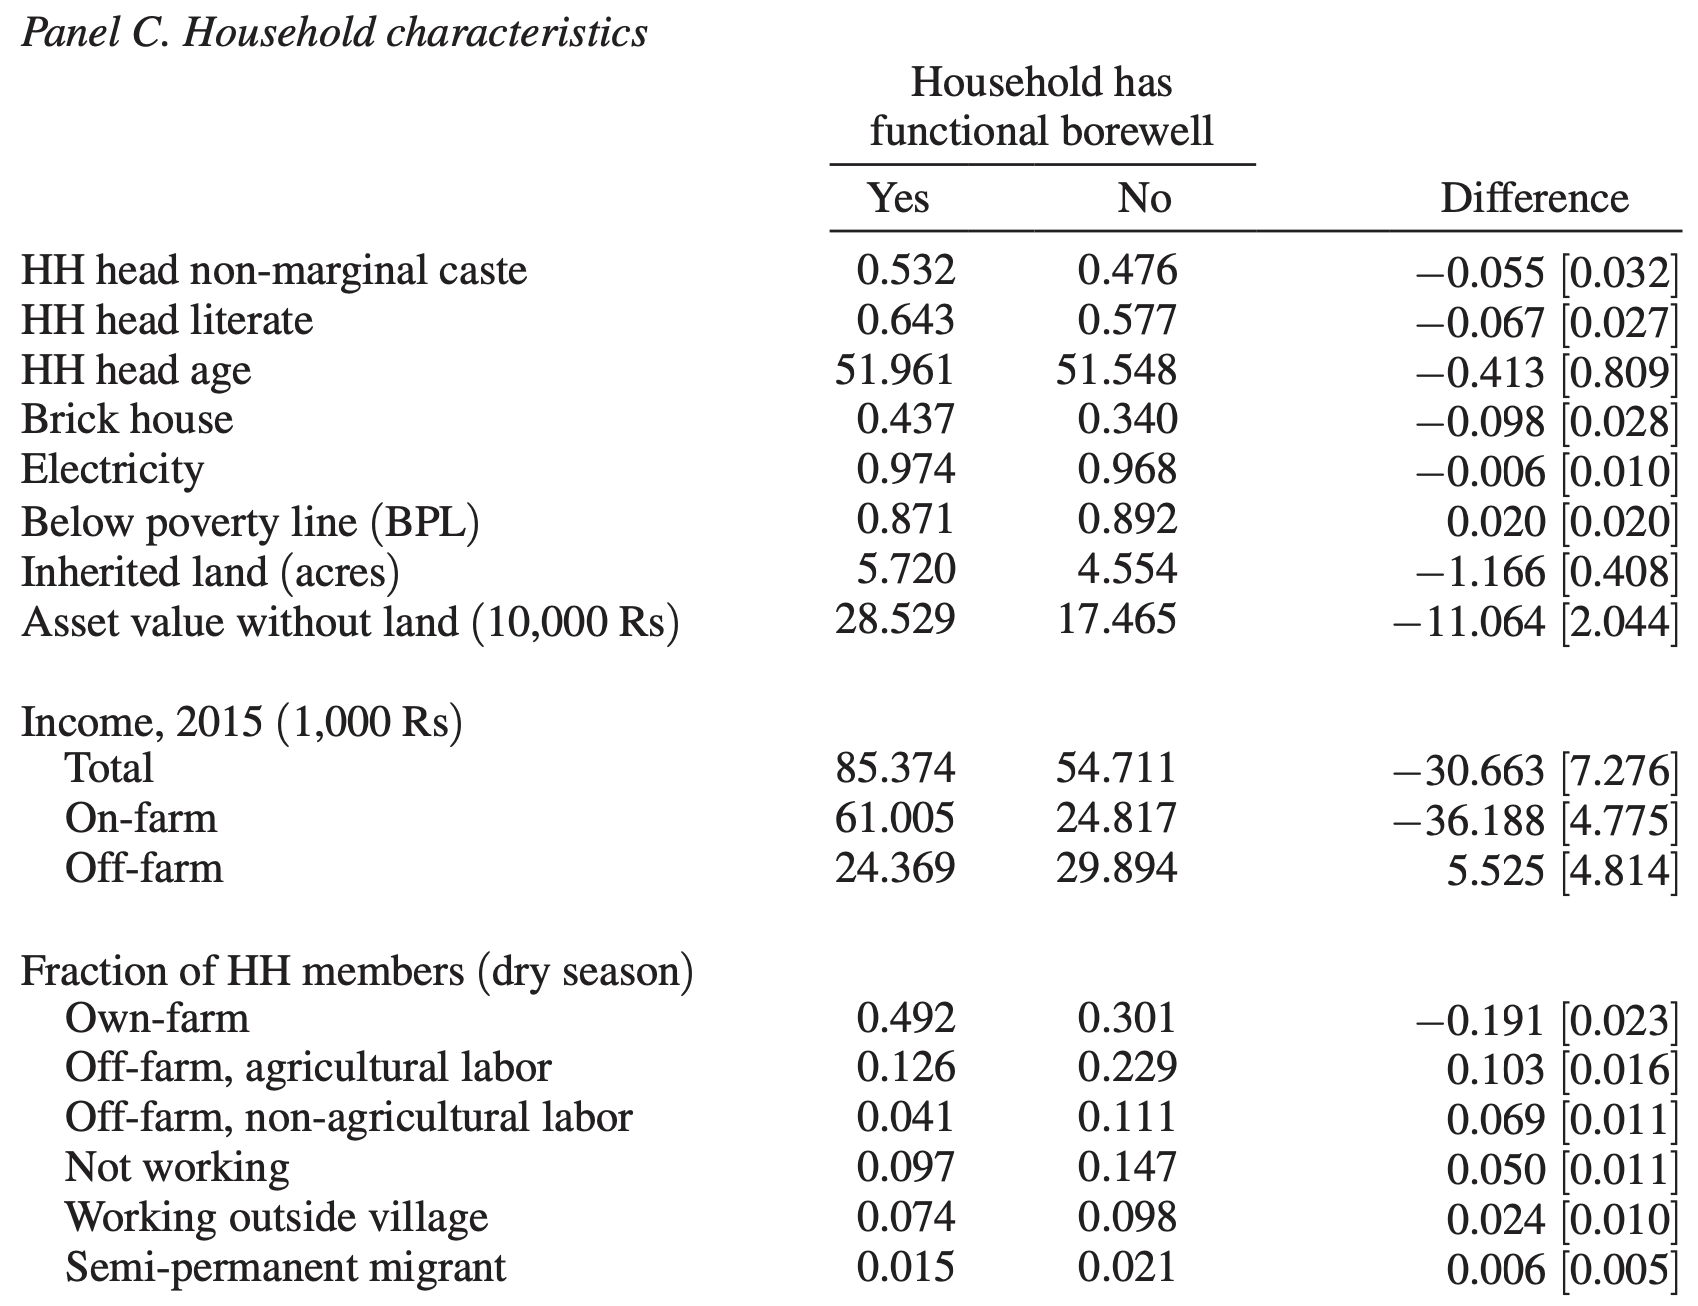
\includegraphics[width=1\textwidth]{table1_c.png}
			\end{figure}
		\end{column}
	\end{columns}
\end{frame}

%=============================================================
\section{Empirical Strategy}
\begin{frame}
	{Empirical Strategy}
	\begin{itemize}
		\item Regression:
	\end{itemize}
	\begin{equation}
		y_{i,v} = \alpha_1 + \underbrace{\alpha_2 F_i}_{\text{effect of borewell failure}} + \underbrace{X_i \Phi}_{\text{household characteristics}} + \underbrace{A_v}_{\text{village fixed effects}} + \underbrace{B_t}_{\text{year fixed effects}} + u_i
	\end{equation}
	\begin{itemize}
		\item Household characteristics include age, caste, literacy, total land inherited
		\item Robustness tests: depth and cost of the first borewell, alternative specs of first borewell age
		\item All regressions incorporate sampling weights for the relative share of HH with/without first borewell in the village
		\item Identifying assumption: conditional on year of drilling, failure of first borewell is exogenous to any other correlates of the outcomes
		\item Remaining determinants of failure primarily depend on highly variable and quasi-random hydrogeological characteristics (such as number of sources the well intersects)
	\end{itemize}
\end{frame}


%=============================================================
\section{Results}
\begin{frame}
	{Results}
	\begin{figure}
		\centering
		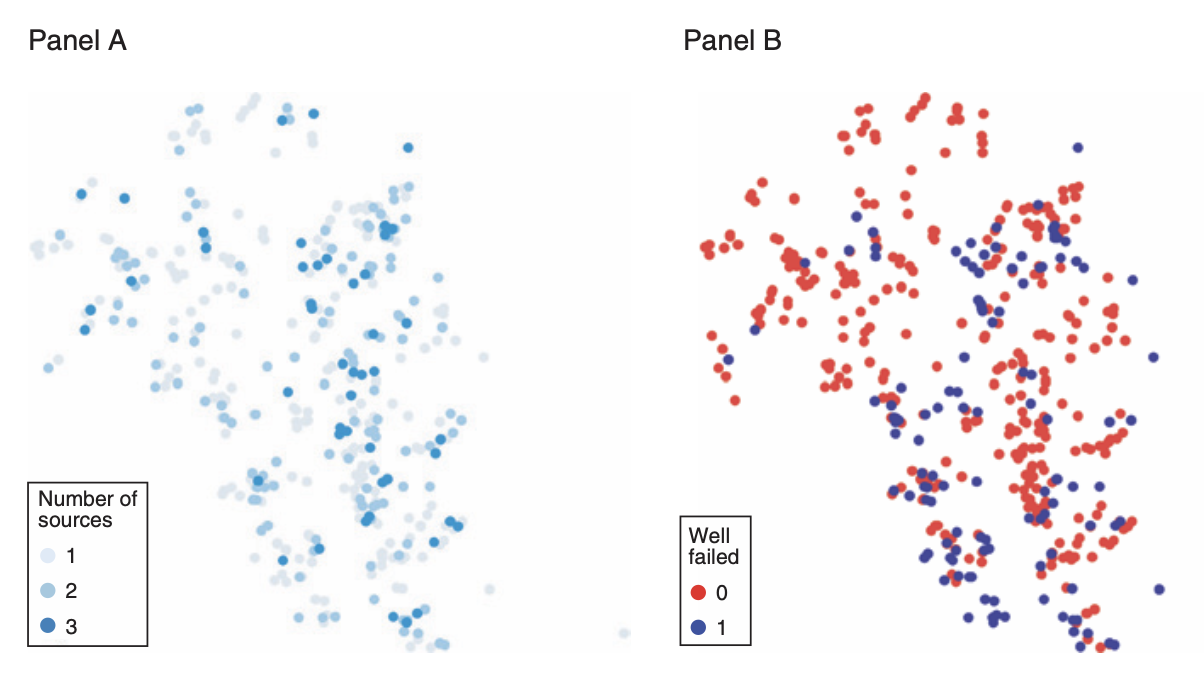
\includegraphics[width=0.8\textwidth]{figure3.png}
	\end{figure}
\end{frame}

%=============================================================
\begin{frame}
	{Results}
	\begin{figure}
		\centering
		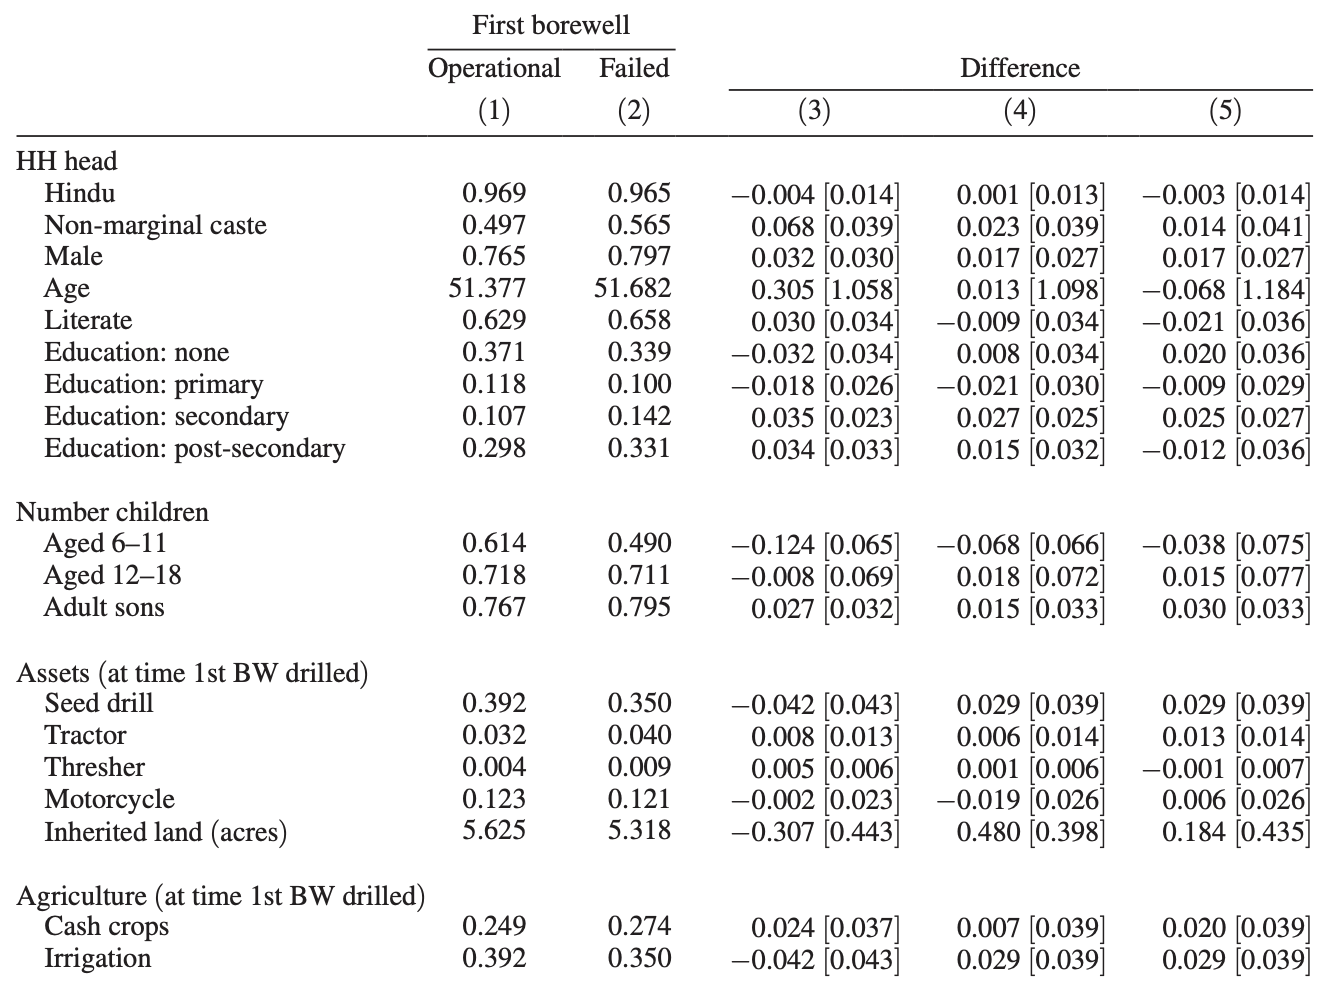
\includegraphics[width=0.65\textwidth]{table2.png}
	\end{figure}
\end{frame}


%=============================================================
\begin{frame}
	{Results}
	\begin{figure}
		\centering
		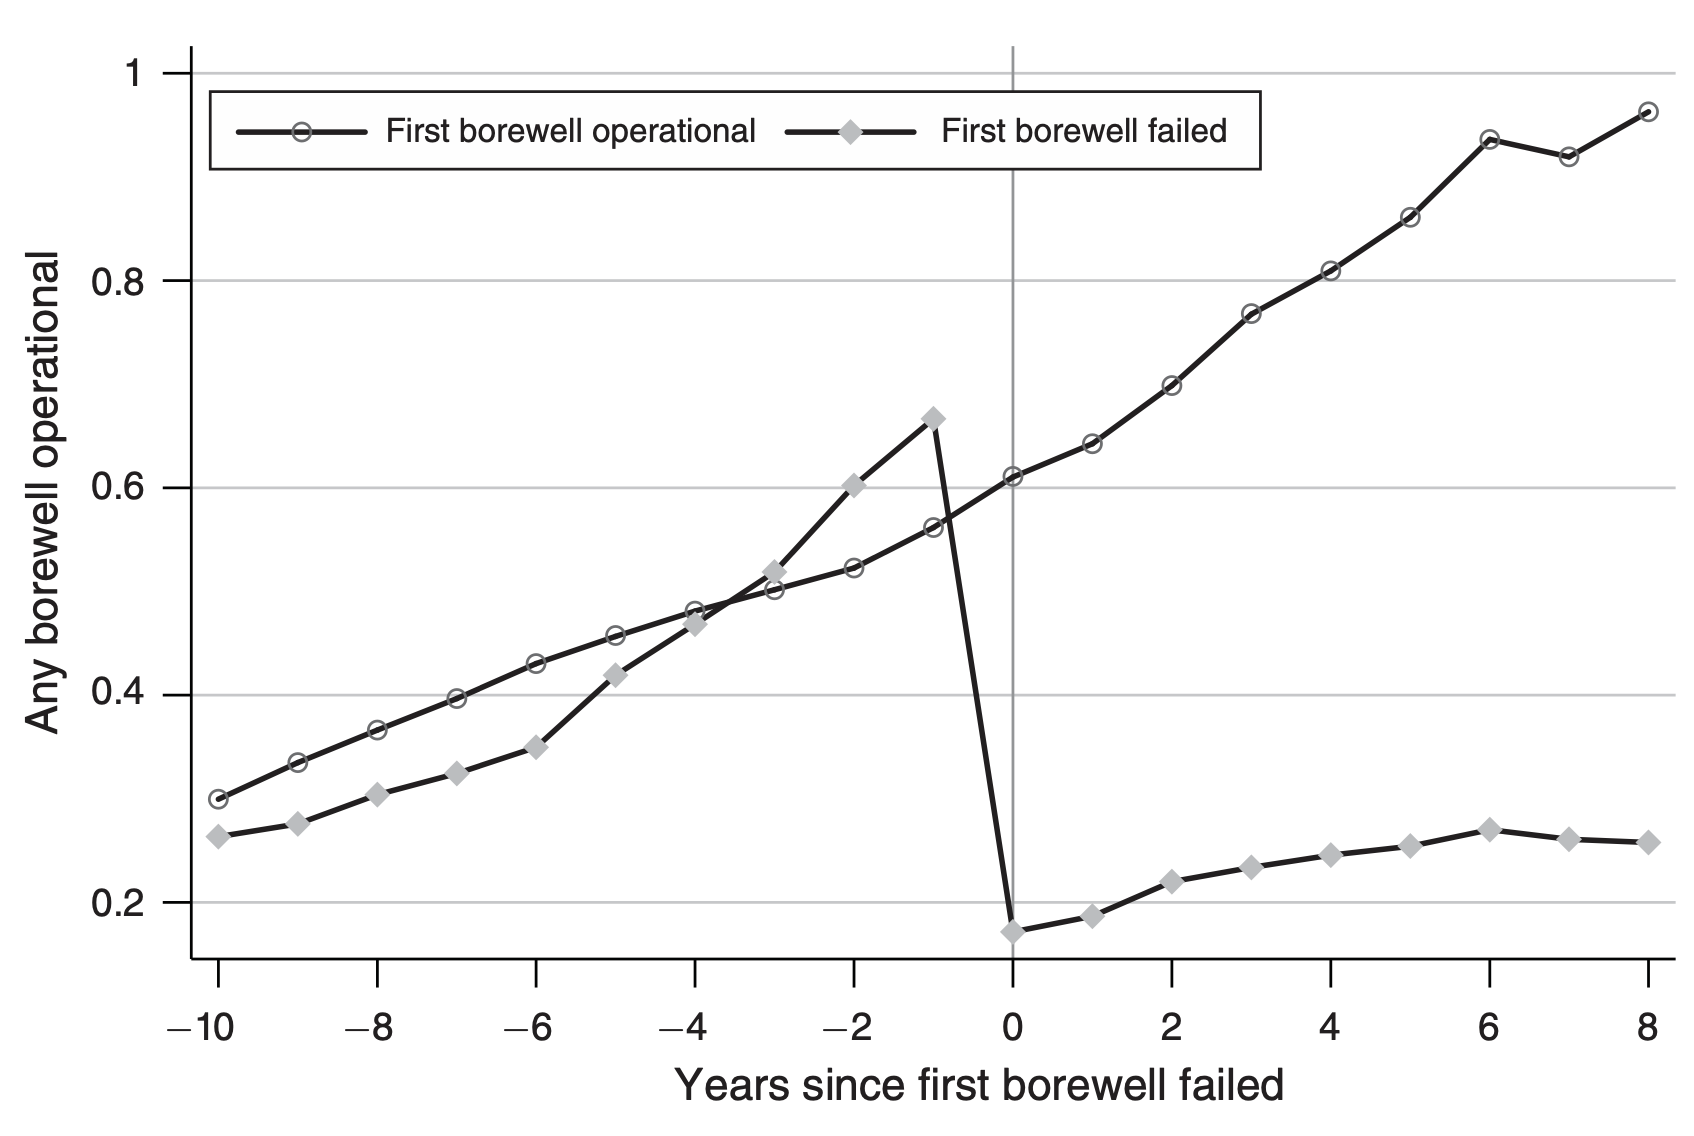
\includegraphics[width=0.7\textwidth]{figure4.png}
	\end{figure}
\end{frame}

%=============================================================
\begin{frame}
	{Results}
	\begin{columns}
		\begin{column}{0.5\textwidth}
			\begin{figure}
				\centering
				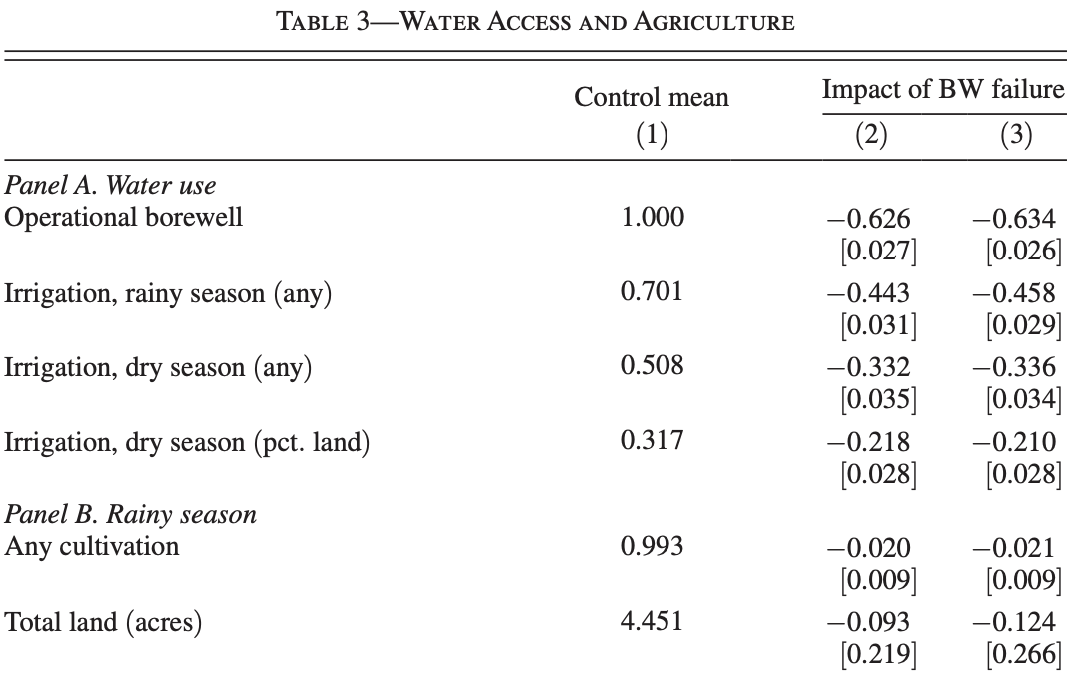
\includegraphics[width=1\textwidth]{table3_a.png}
			\end{figure}
		\end{column}
		\begin{column}{0.5\textwidth}
			\begin{figure}
				\centering
				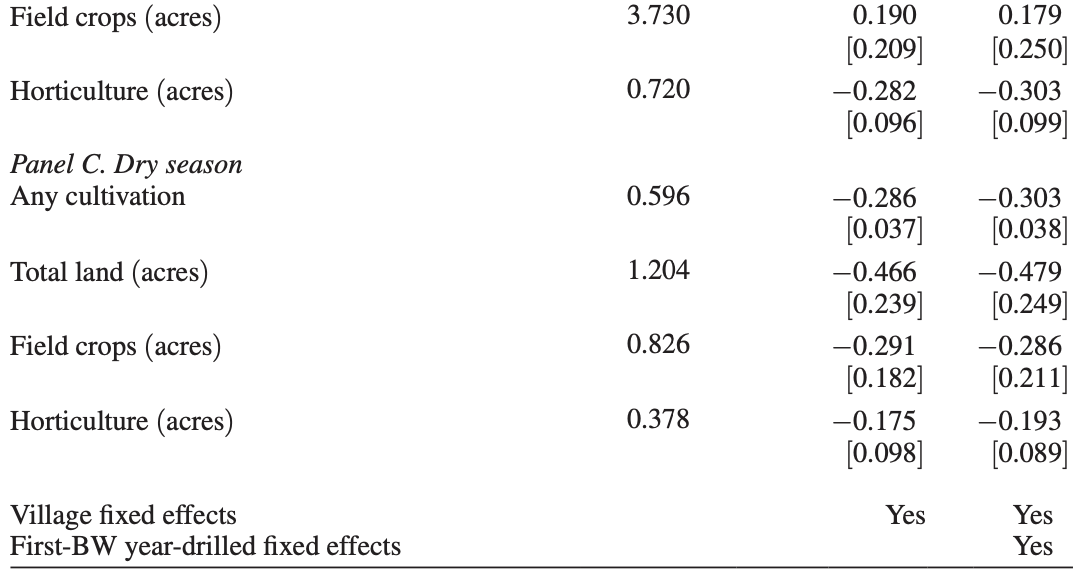
\includegraphics[width=1\textwidth]{table3_b.png}
			\end{figure}
		\end{column}
	\end{columns}
\end{frame}
%=============================================================
\begin{frame}
	{Results}
	\begin{columns}
		\begin{column}{0.5\textwidth}
			\begin{figure}
				\centering
				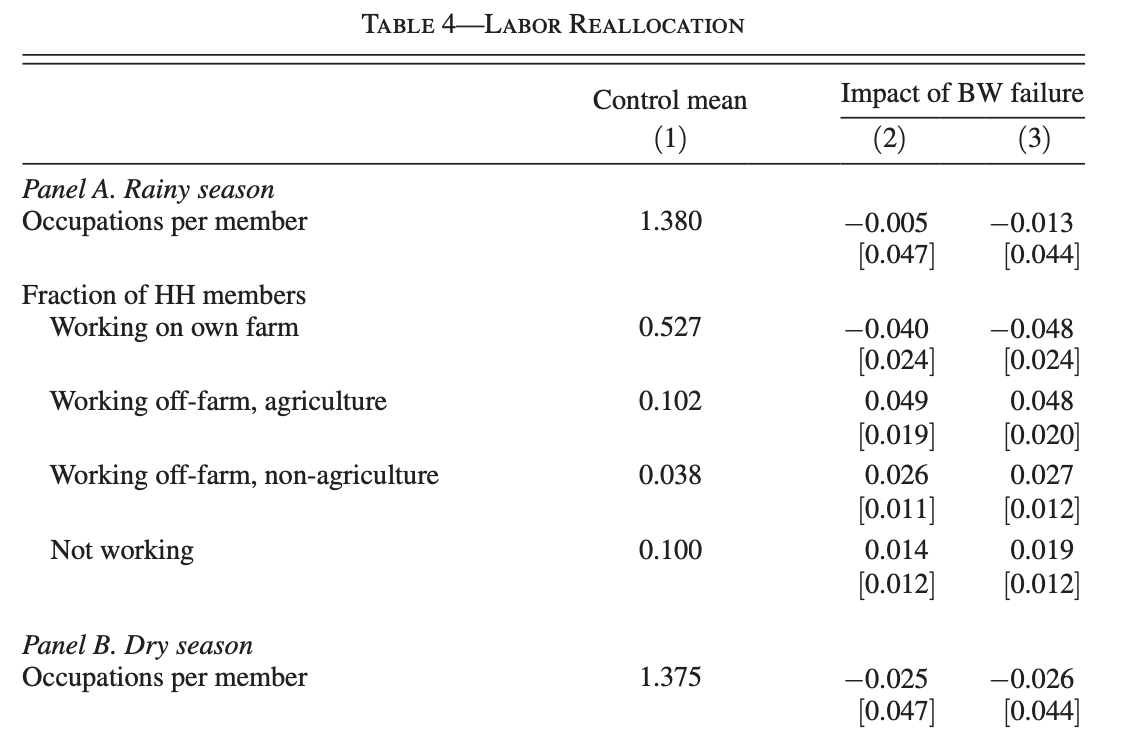
\includegraphics[width=1\textwidth]{table4_a.png}
			\end{figure}
		\end{column}
		\begin{column}{0.5\textwidth}
			\begin{figure}
				\centering
				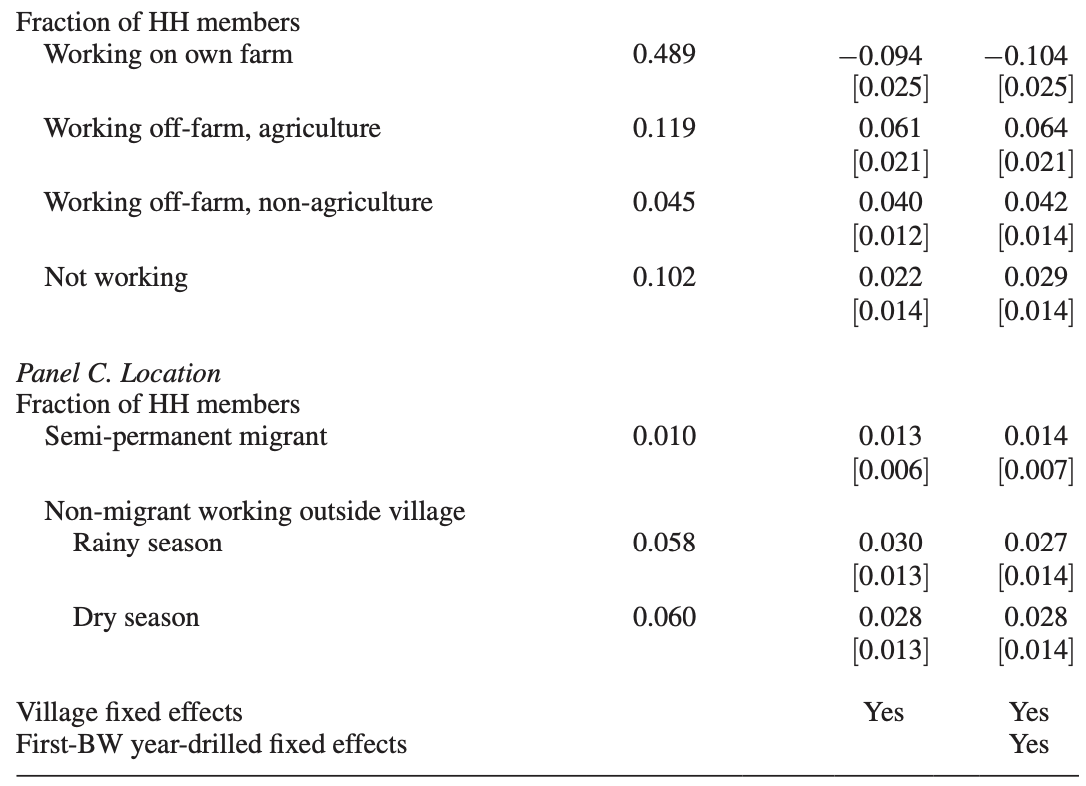
\includegraphics[width=1\textwidth]{table4_b.png}
			\end{figure}
		\end{column}
	\end{columns}
\end{frame}
%=============================================================
\begin{frame}
	{Results}
	\begin{figure}
		\centering
		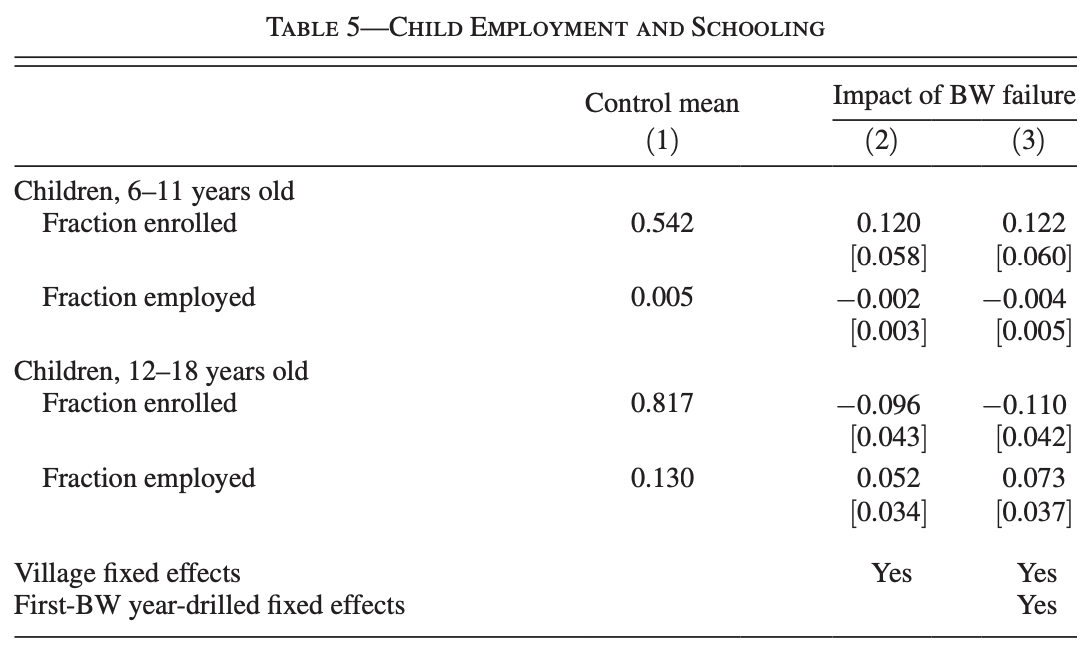
\includegraphics[width=0.7\textwidth]{table5.png}
	\end{figure}
\end{frame}

%=============================================================
\begin{frame}
	{Results}
	\begin{figure}
		\centering
		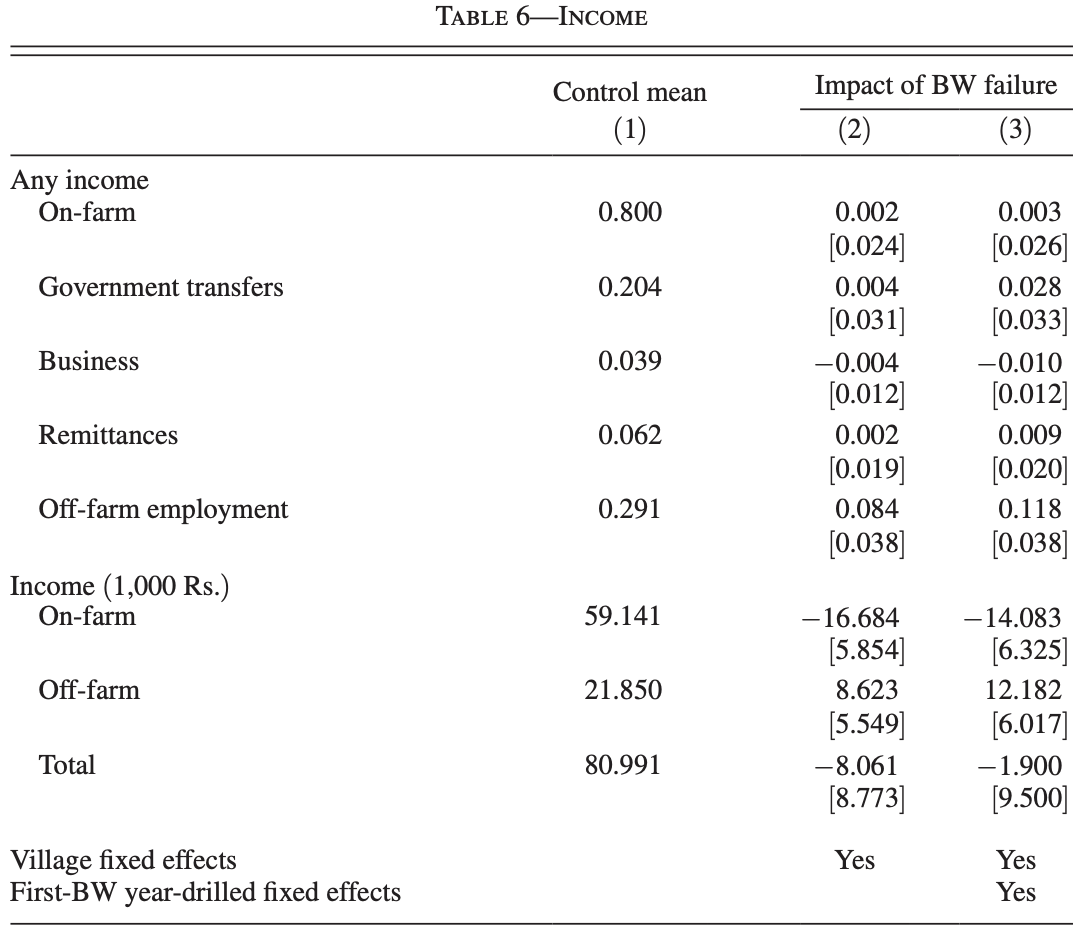
\includegraphics[width=0.56\textwidth]{table6.png}
	\end{figure}
\end{frame}
%=============================================================
\begin{frame}
	{Results}
	\begin{figure}
		\centering
		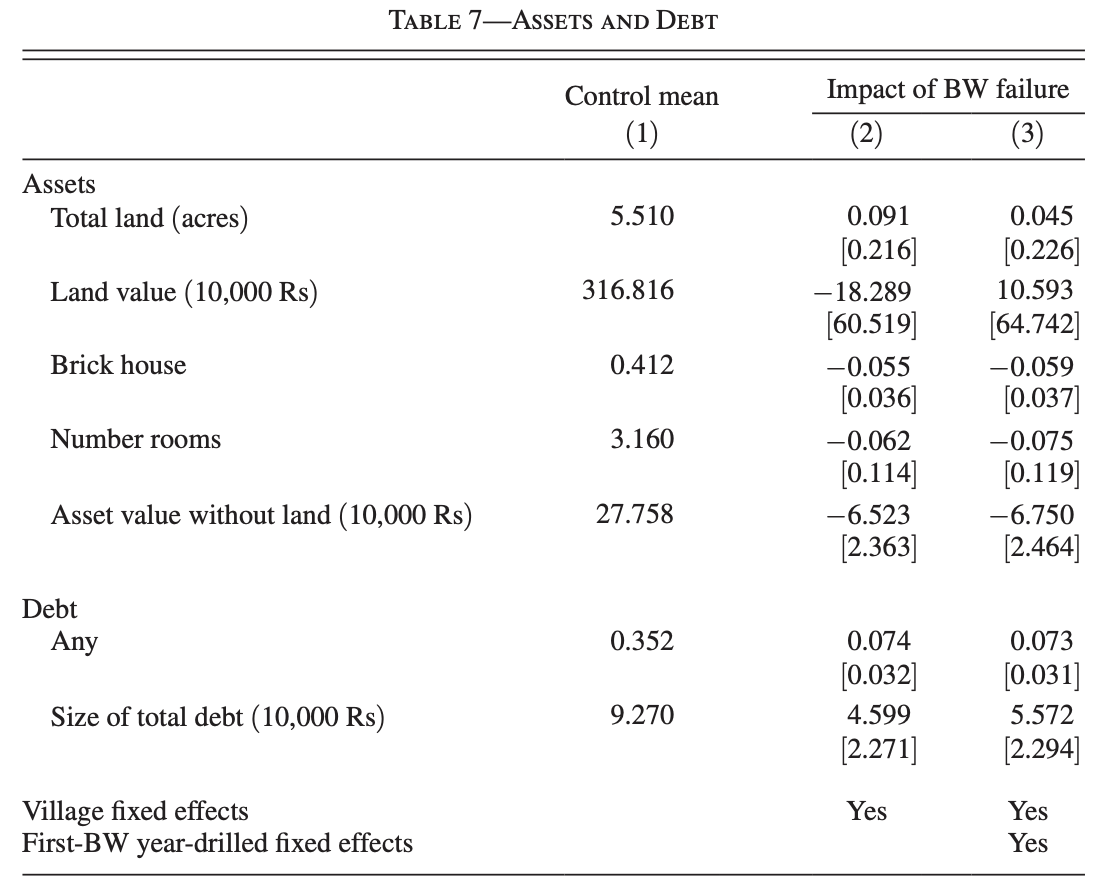
\includegraphics[width=0.6\textwidth]{table7.png}
	\end{figure}
\end{frame}
%=============================================================
\section{Conclusion}
\begin{frame}
	{Conclusion}
	\begin{itemize}
		\item Evidence of long-term impacts of large-scale, permanent environmental deterioration in a developing country
		\item Loss of access to irrigation water reduces agricultural viability with minimal adaptation
		      \begin{itemize}
			      \item Affected land often left fallow or cultivated with low-value crops
			      \item Raises concerns about aggregate food production
		      \end{itemize}
		\item Households offset agricultural income losses by reallocating labor to off-farm employment
		      \begin{itemize}
			      \item Regions with many large firms: higher off-farm employment, slight total income increase
			      \item Regions with few large firms: total income declines slightly
		      \end{itemize}
		\item This adaptation involves trade-offs:
		      \begin{itemize}
			      \item Asset liquidation, debt accumulation, reduced food expenditures
			      \item Lower human capital investments for older children
		      \end{itemize}
	\end{itemize}
\end{frame}


%=============================================================
\section{Thesis}
\begin{frame}{Thesis}
	\begin{columns}
		% Left column
		\begin{column}{0.7\textwidth}
			\begin{itemize}
				\item Micro Irrigation (drip and sprinkler systems) can improve agricultural efficiency by saving 30—70 percent of water compared to conventional methods
				\item Adoption levels remain low in India due to a lack of incentives for efficiency; water and electricity is unpriced or heavily subsidized
				\item All-India dataset: village-level panel data from the Minor Irrigation Census (1993—2017), used to assess adoption patterns and water scarcity correlations; will be merged with climatic data, socio-economic indicators, and satellite-based irrigation estimates
				\item Gujarat dataset: high-resolution data tracks 400,000 geo-referenced MI adopters (2006—2013), includes detailed subsidy variations, enabling analysis of adoption determinants, social learning effects, and water conservation outcomes
			\end{itemize}
		\end{column}

		% Right column
		\begin{column}{0.3\textwidth}
			\centering
			\begin{figure}
				\centering
				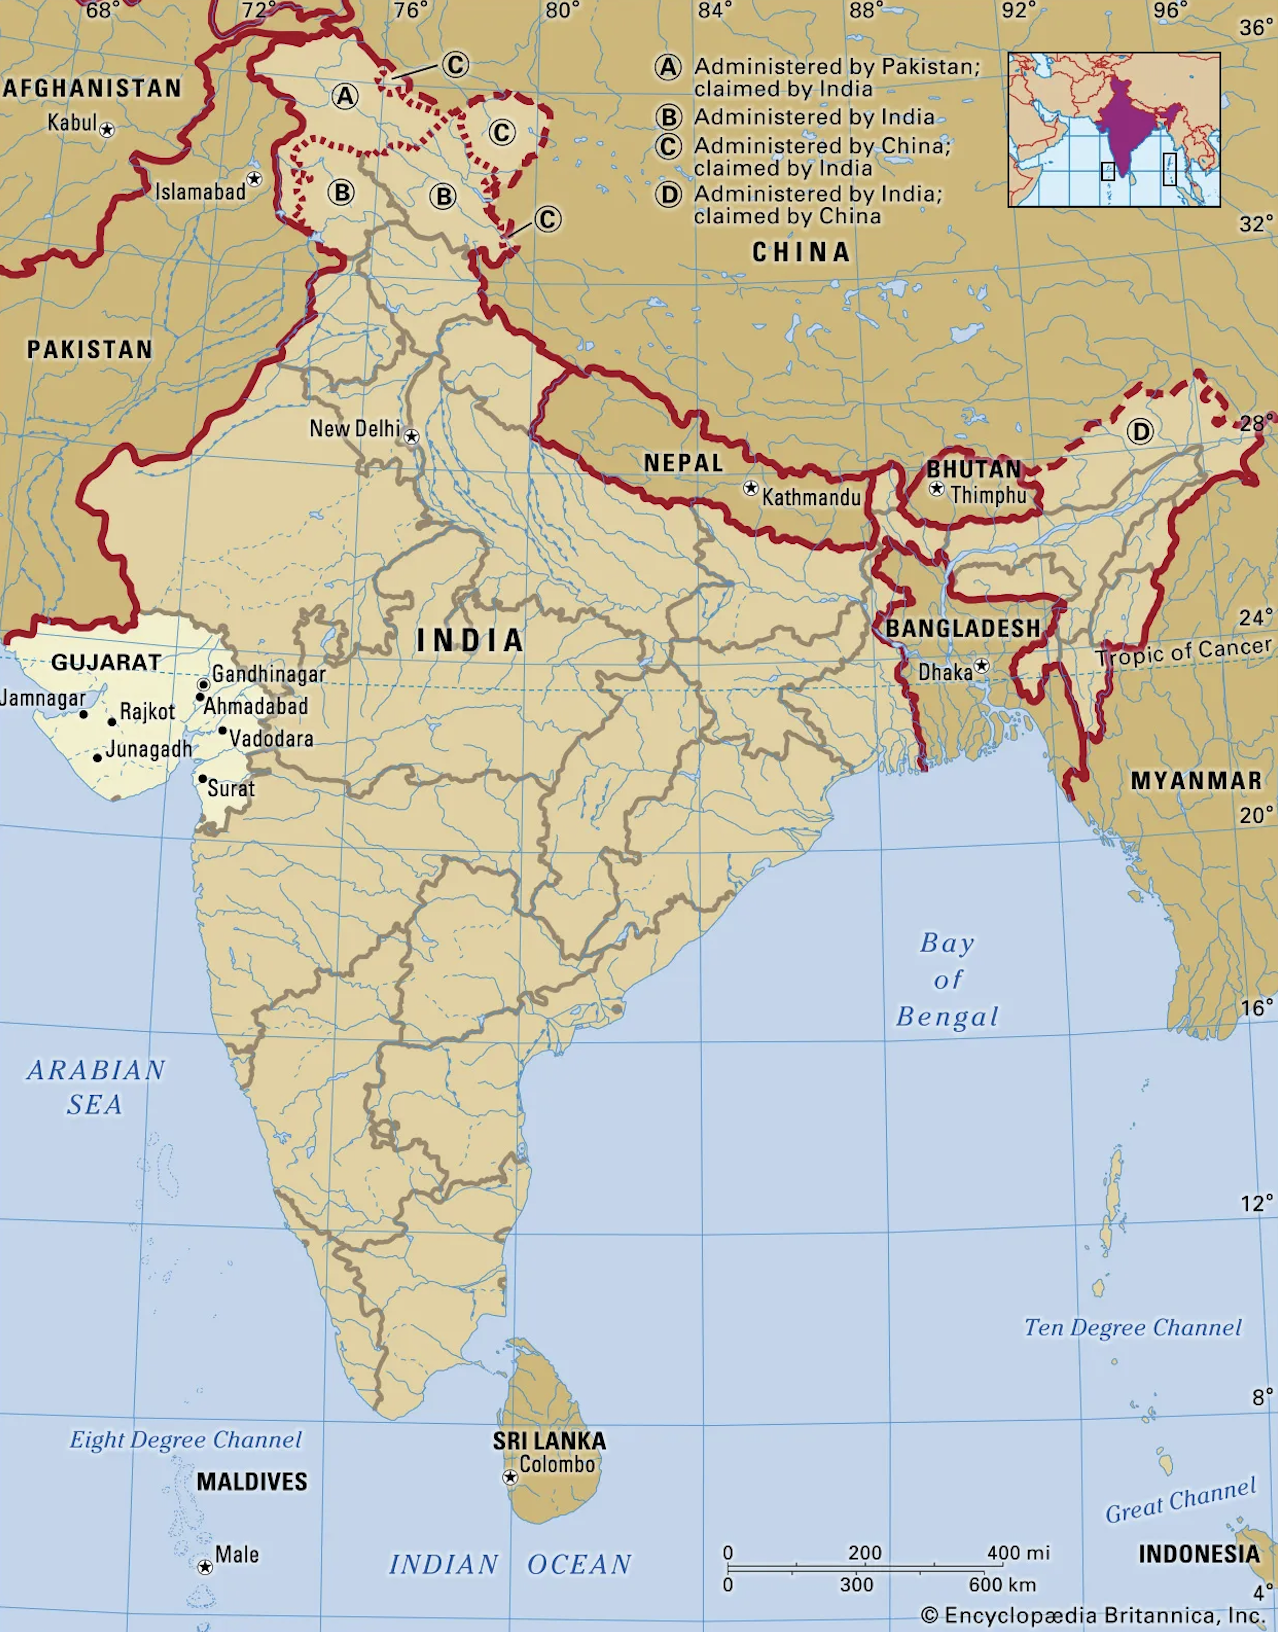
\includegraphics[width=1\textwidth]{gujarat.png}
				\caption{Map of India}
			\end{figure}
		\end{column}
	\end{columns}
\end{frame}
%=============================================================

\begin{frame}
	{Thesis}
	\begin{itemize}
		\item Working Hypotheses:
		      \begin{enumerate}
			      \item Adoption rates are correlated, across villages and farmers, with indicators of economic development and water scarcity, and these correlations are higher at early stages of diffusion. Earlier adopters are larger farmers, but MI diffuses to smaller farmers in the village over time.
			      \item Variation in water scarcity has causal impacts on the rate of adoption.
			      \item Variation in (subsidy driven) MI cost has causal impacts on the rate of adoption and particularly by smaller farmers.
			      \item Subsidized adoption has spillover effects on adoption in adjacent areas (presumably through social learning), but these are limited by crop type and social groups (castes).
			      \item Subsidized adoption has varying effects on water and power use for pumping, depending on the extent of overall irrigation coverage in the village and the existence of informal water markets.
		      \end{enumerate}
	\end{itemize}
\end{frame}


%=============================================================

\end{document}


